\documentclass{book}

\usepackage{amsmath}
\usepackage{graphicx}
\usepackage{amsthm}
\usepackage{amsfonts}
\usepackage{amssymb}
\usepackage{mathrsfs}
\usepackage{tikz}
\usepackage{fontspec}
\usepackage{imakeidx}
\usepackage{listings}

\title{Motion Of Entities \\ {\small{An Algebraic Approach} \\ {\small{GTM Graduate Text In Minecraft 784}}}}

\author{2717498529 @ CNU}
\date{May 7th, 2026}

\newtheorem{definition}{Definition}
\newtheorem{lemma}{Lemma}
\newtheorem{theorem}{Theorem}
\theoremstyle{remark}\newtheorem*{remark}{Remark}

\DeclareMathOperator*{\argmin}{arg\,min}

\definecolor{gtmyellow}{HTML}{F9CA04}

\makeindex

\begin{document}

\setsansfont{QTAtchen}

\begin{tikzpicture}[remember picture, overlay]
	\fill[white](current page.south east)rectangle (current page.north west);
	\coordinate (A) at (current page.south west);
	\coordinate (B) at (current page.north west);
	\coordinate (C) at ([yshift=0.95\textheight]A);
	\coordinate (D) at ([yshift=0.01\textheight]A);
	\coordinate (E) at (D-|current page.south east);
	\coordinate (F) at (C-|current page.north east);
	\node [yscale=1.7, scale=8, color=gtmyellow] at (6.5, 0.8){\normalfont\sffamily\bfseries{GraduateTexts}};
	\node [yscale=1.7, xscale=1.23, scale=8, color=gtmyellow] at (6.5,-2.8){\normalfont\sffamily\bfseries{InMinecraft}};
	\fill[gtmyellow] (C)--(D)-- (E) -- (F) -- cycle;
	\node [scale=3.8] at (6.5,-8){\fontencoding{T1}\fontfamily{ptm}\bfseries\selectfont The Crazy Authors };
	\node [scale=5] at (6.5,-10.5){\fontencoding{T1}\fontfamily{ptm}\bfseries\selectfont Motion Of Entities };
	\node [scale=3] at (6.5,-13){\fontencoding{T1}\fontfamily{ptm}\bfseries\selectfont An Algebraic Approach};

	\node[scale=2] at ([yshift=2cm, xshift=-4.0cm]current page.south){{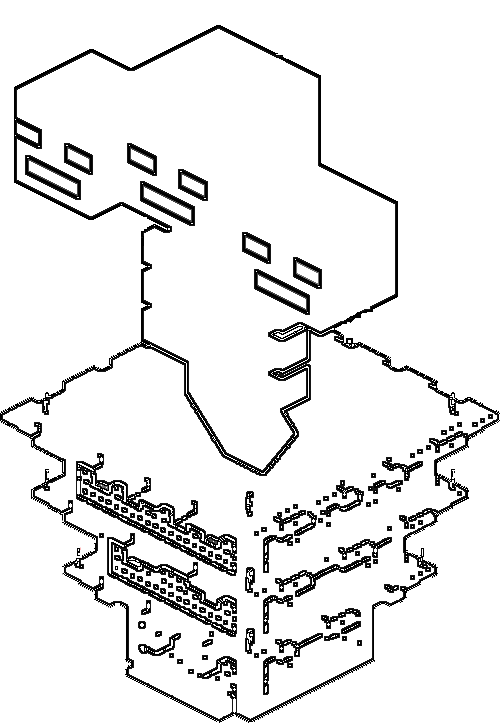
\includegraphics[height=1cm]{autumner.png}}};
	
	\node[scale=2.5] at ([yshift=2cm, xshift=0.6cm]current page.south){{\bf Autumner Press}};
\end{tikzpicture}

\newpage

\begin{tikzpicture}[remember picture, overlay]
	\fill[white](current page.south east)rectangle (current page.north west);
	\node[scale=2] at ([xshift=3cm, yshift=-3cm]current page.north){{\bf Graduate Text in Minecraft 784}};
\end{tikzpicture}

\frontmatter

\maketitle

\chapter{Forewords}

As an important part of technological Minecraft, motion of entities has always been one of central topics in the community, and countless well-known applications (e.g. pearl cannons, border traveling and item transportation) have resulted. However, there are rarely dedicated discussion on specific mechanisms for the motion itself, compared to the hottest topics like block updates and mob spawning which has been thoroughly explained, experimented and applied by numerous researchers and engineers.

Sets of kinematic formulas for specific types of entities of interest like TNTs and terminologies like momentum were put into usage as early as middle 2010s and field experts like cannon designers had their own empirical and mathematical models on the topics they concerned at that time.

However, a unified framework isn't formulated until July 2021 when lovexyn0827 released their 70k words dissertation, the first complete discussion on our topic ever publicly available, which extensively covers from fundamental theoretical grounding and complete kinematic formulas different update orders, to detailed analysis on a range of mechanisms and almost every negligible corner cases ever practically related. Despite its fundamental contribution to theorists, it is commonly considered "too hard to begin with" due to its complex monolithic theoretical framework, and its sheer tediousity is enough to scare readers off. Nevertheless, it marks a mew era of researches on motion of entities.

A newer book releases a few weeks ago by MCS\&E has adopted an axiomized approach to present mechanisms in a rigorous while pedagogically viable way. Asides from inheriting lovexyn0827's theoretical framework with radical optimization, it has employed its on educational strategies and introduced field analysis to its analytical toolkit to gain new a new insight by visualization and calculation. Well-structured and self-contained though, it lakes proper treatment to many topics like dimensionalities (a.k.a. units), collision detection, floating point errors and piston push, which is essential in engineering practices. Besides, it is suspected to abuse fancy mathematical concepts simply to show off, and ignored capture the discrete nature of Minecraft before diving to continuous approximations too deep, inspect of which its asymptotic analysis has contributed much to practices.

Therefore, we are writing the book to suggest a complete and mathematical rigorous framework applicable to both continuous approximation and machinery reality. Our approach to kinematics is:

\begin{enumerate}
	\item To devise a unified framework compatible with any algebraic structure with arithmetics;
	\item Study two special cases,
	\begin{enumerate}
		\item One for real numbers, to calculate and approximate;
		\item Another for floating point numbers, to bound errors;
	\end{enumerate}
	\item Combine both to establish a approximation along with a (hard or probabilistic) bound, for "physically" rigorous analysis.
\end{enumerate}

Furthermore, a universal model for world and ticking is established, and will lead us to a novel paradigm of game mechanism analysis.

\begin{flushright}
	May 14th, 2026
	
	2717498529 @ Capital Normal University
\end{flushright}

\tableofcontents

\mainmatter

\chapter{Foundations}

\section{General Notations}

\begin{definition}
	The $k$-th component of a list / vector $L$ is denoted $L[k]$.
\end{definition}

\begin{definition}
	The length of a list / vector $L$ is denoted $|L|$.
\end{definition}

\begin{definition}
	The concatenation of a finite sequence of lists / vectors $L_1, \dots, L_k$ is denoted $\operatorname{concat}(L_1, \dots, L_k)$.
\end{definition}

\begin{definition}
	Given a list $L$, set $\bigcup_{k = 1}^{|L|} \{L[k]\}$ shares the same notation as $L$.
\end{definition}

\subsection*{Exercises}

Too easy to assign exercises.

% ============================ The End Of Section ============================

\section{Motion Operators}

\begin{definition}
	 A \index{unit group}{\bf{unit group}} $\left<U\right>$ is the abelian group generated by $U$, the {\bf{elementary unit set}}, all of whose elements has an infinite order. An element in an unit group is a \index{unit}{\bf{unit}}.
\end{definition}

\begin{definition}
	An \index{united algebra}{\bf{united algebra on $A$ with unit $u$}}, notably $A_u$, is an algebraic structure of ordered pairs $<m, u>$, where $m \in A$ , $u\in U$ for some unit group $U$ and $A$ is an algebraic structure. An element in an united algebra is a \index{united value}{\bf{united value}}. Its left and right component are called its \index{magnitude}{\bf{magnitude}} $\mu(<m, u>)$ and \index{unit}{\bf{unit}} $\upsilon(<m, u>)$ respectively.
	
	If addition and / or abstraction are defined on $A$, they are automatically defined on $A_u$ by $<m_1, u> \pm <m_2, u> = <m_1 \pm m_2, u>$.
	
	If multiplication is defined on $A$, it is also defined between elements in two possibly different united algebras on $A$ as $<m_1, u_1><m_2, u_2> = <m_1 m_2, u_1 u_2>$, where $u_1$ and $u_2$ is multiplied with the binary operator on $U$. If there is a multiplicative inverse $m^{-1}$ of $m$ in $A$, $<m, u>^{-1} = <m^{-1}, u^{-1}>$
	
	For $u_1$ and $u_2$ in the same unit group and $A$ with a multiplicative identity $1_A$, the \index{transition unit}{\bf{transition unit from $A_{u_1}$ to $A_{u_2}$}} is $<1_A, u_1^{-1}u_2>$.
\end{definition}

\begin{remark}
	United algebra is not an algebra being "united" but an algebraic structure with units.
\end{remark}

\begin{remark}
	Note that addition is closed on $A_u$ but multiplication is not necessarily.
\end{remark}

\begin{remark}
	If the unit of an united value is the identity of underlying unit group, it is regarded to equal its magnitude for convenience. If the magnitude of an united value is the additive identity and multiplicative zero, then one is free to take any value for its unit to make expressions involved sensible.
\end{remark}

\begin{definition}
	Given an algebraic structures $F$ on which addition and multiplication is defined and with an additive and multiplicative identity, two units $u_x$, $u_v$ in the same unit group $U$, the \index{entity state space}{\bf{ $n$-dimensional entity state space on $F$ with unit $u_x$ and $u_v$}}, denoted $S_{F, u_x, u_v, n}$ and abbreviated {\bf{state space}}, is the set of ordered pairs of two $n$-tuples, with the left component in $F_{u_x}^n$ and the right one in $F_{u_v}^n$.
	\begin{equation*}
		S_{F, u_x, u_v, n} = \{ <x, v> : x \in F_{u_x}^n \land v \in F_{u_v}^n\}
	\end{equation*}
\end{definition}

\begin{remark}
	As a idealized model, we define the \index{continuous entity state space}{\bf{$n$-dimensional continuous entity state space}} as $C_n = S_{\mathbb{R}, 1_U, 1_U, n}$, where $\mathbb{R}$ is the field of real numbers with conventional addition and multiplication and $1_U$ is the identity in an unit group $U$. Note that $C_n$ is the set of ordered pairs of $n$-dimensional real vectors.
\end{remark}

\begin{remark}
	The definition has imposed a minimized requirement on qualified $F$'s. This decision, although may result in a overly high level of abstraction, allows the floating point arithmetic which is done on real computers and Minecraft instances to our framework.
\end{remark}

\begin{remark}
	One is free to believe $F_u^n = (F_u)^n$ or $(F^n)_u$.
\end{remark}

\begin{remark}
	Two distinct united algebraic structures are involved in the definition to prohibit direct addition / subtraction between objects with different dimensions (in other words, for different physical concepts). Multiplication is the only natural legitimate way in which they interact.
\end{remark}

\begin{definition}
	An element in a state space is an \index{entity state}{\bf{entity state}}.
\end{definition}

\begin{definition}
	The left component of an entity state $S$ is the position component of the it, denoted $P(S)$. The right component of $S$ it the velocity component of it, denoted $V(S)$.
\end{definition}

\begin{remark}
	Any ordered pair of $3$-dimensional real vector, $<(x, y, z), (v_x, v_y, v_z)>$ with $x, y, z, v_x, v_y, v_z \in \mathbb{R}$ is an entity state in $C_3$.
\end{remark}

\begin{definition}
	Given a state space $S$, a \index{motion operator}{\bf{motion operator on $S$}} is a function $f: S\to S$.
\end{definition}

\begin{definition}
	Given a $n$-dimensional state space $S$ on $F$ with units $u_x$ and $u_v$, there are three families of \index{basic elementary motion operator}{\bf{basic elementary motion operators}}, defined as follows
	
	\begin{enumerate}
		\item {\index{movement operator}\bf{Movement operators}} $\{M_{t}: M_{t_0}<x, v> = <x + vt, v> \land t \in T\}$;
		\item {\index{acceleration operator}\bf{Acceleration operators}} $\{A_{I}: A_{I}<x, v> = <x, v + I> \land I\in F_{u_v}^n\}$;
		\item {\index{drag operator}\bf{Drag operators}} $\{D_k: D_k<x, v> = <x, kv> \land k\in U\}$
	\end{enumerate}
	
	Where $T = \{<m, u_v^{-1}u_x>: m\in F\}$ and $U = \{<m, u_x^{-1}u_v>: m\in F\}$.
	
	An motion operator is \index{elementary motion operaror}{\bf{elementary}} if it is the composition of some finite lists of these operators. 
	
	Furthermore, an elementary motion operator is {\bf{simple}} if there exists one of its factorization as a finite composition of basic elementary motion operators containing at most one movement operator.
\end{definition}

\begin{remark}
	Component-wise addition and scalar multiplication is implied in the definition.
\end{remark}

\begin{remark}
	One would prefer to name acceleration and drag operators as additive and decaying operators respectively.
\end{remark}

\begin{theorem}
	The set of all elementary motion operators except $D_0$ on a state space on a division ring is a group under function composition.
\end{theorem}

\begin{remark}
	We denote such group as $\mathcal{E}_S$, where $S$ is the state space mentioned.
\end{remark}

\begin{proof}
	Closure and associativity is trivial, and the identity is trivially $M_0 = D_0 = D_1$. For a inversibility, consider the inverse of basic elementary motion operators:
	
	\begin{equation*}
		\begin{matrix}
			M_{t}^{-1} = M_{-t}&
			A_{I}^{-1} = A_{-I}&
			D_{k}^{-1} = D_{k^{-1}}
		\end{matrix}
	\end{equation*}
	
	Therefore, given an elementary motion operator $f: f_1 \circ \cdots \circ f_n$, where $f_1, \dots, f_n$ are basic elementary motion operators, its inverse is
	
	\begin{equation*}
		f^{-1} = f_n^{-1} \circ \cdots \circ f_1^{-1}
	\end{equation*}
	
	As one can verify.
\end{proof}

\begin{remark}
	We are adopting left composition in this book, that is, $(f \circ g)(x) = g(f(x))$. It is so that the visual order of a long sequence of motion operators will be consist with the order in which they are applied.
\end{remark}

\begin{definition}
	Given a state space $S$, an \index{inspect function}{\bf{inspect function}} is a function $f: S \times S \to \{0, 1\}$ such that:
	
	\begin{enumerate}
		\item $x = y \implies f(x, y) = 1$;
		\item $f(x, y) = f(y, x)$;
		\item $f(x, y) = 1 \land f(y, z) = 1 \implies f(x, z) = 1$.
	\end{enumerate}
	
	Two entity states $S_0, T_0$ is \index{$f$-equivalent}{\bf{$f$-equivalent}} if $f(S_0, T_0) = 1$, denoted $S_0 \overset{f}{\sim} T_0$.
\end{definition}

\begin{remark}
	It's easy to see that $f$-equivalence is an equivalence relation.
\end{remark}

\begin{remark}
	The \index{natural inspect function}{\bf{natural inspect function}} is defined as $\nu : (x, y) \mapsto x = y$. It's easy to see that if $\nu$ maps a pair of entity states to 1, so do any other inspect function. For comparisons on specific components, we have the {\bf{natural inspect function for position}} $\nu_p: (x, y) \mapsto P(x) = P(y)$ and the one for velocity $\nu_v: (x, y)\mapsto V(x) = V(y)$.
\end{remark}

\begin{definition}
	An \index{application of inspect function}{\bf{application of inspect function}} $f$ on $S$ is a function defined by tuple $<m, n, f>$ with $m, n \in \mathbb{N}$ that maps an entity state $S_0\in S$ along with any two lists of motion operators, $f_1, \dots, f_M$ and $g_1, \dots, g_N$ with $m > M$ and $n > N$, to a boolean value
	
	\begin{equation*}
		<m, n, f>: (S_0, f_1, \dots, f_M, g_1, \dots, g_N) \mapsto (f_1 \circ \cdots \circ f_M)(S_0) = (g_1 \circ \cdots \circ g_M)(S_0)
	\end{equation*}
	
	Given the lists of motion operators defined above, $\underline{f}$, a function from $S_0$ to $\{0, 1\}$ defined by tuple $<M, N, f>$, is the \index{tail application}{\bf{tail application of $f$ on $f_1, \dots, f_M$ and $g_1, \dots, g_N$}}.
\end{definition}

\begin{remark}
	Tail applications test the ultimate equivalence of two sequences of motion operators.
\end{remark}

\begin{definition}
	Given a set $A$ of inspect function applications and state space $S$, two sequence of motion operators, $f_1, \dots, f_M$ and $g_1, \dots, g_N$, are {\bf{$A$-equivalent}} provided that
	
	\begin{equation*}
		\forall \alpha\forall S_0 (\alpha\in A \land S_0 \in S \implies\alpha(S_0, f_1, \dots, f_M, g_1, \dots, g_N) = 1)
	\end{equation*}
	
	In particular, given a set $F$ of inspection functions, if $A$ is the set of tail applications on $f_1, \dots, f_M$ and $g_1, \dots, g_N$ of all inspect functions in $F$, the two lists are \index{$F$-tail equivalent}{\bf{$F$-tail equivalent}} If $F = \{\nu\}$, the two lists are simply \index{tail equivalent}{\bf{tail equivalent}}; if $F = \{\nu_p\}$, the two list are {\bf{positionally tail equivalent}}; and if $A = \{\nu_v\}\}$, the two list are {\bf{velocitically tail equivalent}}.
\end{definition}

\begin{theorem}
	For any set $A$ of inspect function applications, $A$-equivalence is an equivalence relation.
\end{theorem}

\begin{remark}
	If both lists contains exactly one motion operator, say $f$ and $g$ respectively, then they said to be $A$-equivalent as this notation won't cause confusion.
\end{remark}

\begin{remark}
	The existence of $A$-equivalence classes would follow. We take the notation $F / A$ for the set of all A-equivalent classes in a set of motion operators $F$ and the notation of $\overline{f}$ for the class containing $f$.
\end{remark}

\begin{proof}
	Exercise.
\end{proof}

\begin{theorem}\label{thm:f-equiv-iff-tail-equiv}
	Two lists of motion operators on $S$, $f_1, \dots, f_M$ and $g_1, \dots, g_N$, are $\{f\}$-tail equivalent if and only if $(f_1 \circ \cdots \circ f_M)(S_0)$ and $(g_1 \circ \cdots \circ g_N)(S_0)$ are $f$-equivalent for all $S_0\in S$.
\end{theorem}

\begin{proof}
	Trivial.
\end{proof}

\begin{theorem}
	For any set $A$ of inspect function applications and $B\subset A$, two lists of motion operators are $B$-equivalent if they are $A$-equivalent.
\end{theorem}

\begin{proof}
	Immediate from the definition.
\end{proof}

\begin{theorem}
	Given a set $A$ of inspection functions on $S_{F, n}$ with $F$ being a division ring, then the set $\mathcal{E}_S / A$ of all $A$-equivalence classes in $\mathcal{E}_S$ forms a group under the binary operator $\circ$: 
	
	\begin{equation*}
		\overline{f} \circ \overline{g} \mapsto \overline{f \circ g}
	\end{equation*}
	
	Where $f, g \in \mathcal{E}_S$. 
	
	Furthermore, there is an homomorphism $\pi_A: \mathcal{E}_S \to \mathcal{E}_S / A$.
\end{theorem}

\begin{proof}
	Trivial.
\end{proof}

\begin{theorem}
	Given a state space $S$ on a division ring, the subset $\{f: f\in \mathcal{E}_S \land f \text{ is }A\text{-equivalent to } M_0\}$ of $\mathcal{E}_S$ is a normal subgroup in $\mathcal{E}_S$.
\end{theorem}

\begin{proof}
	Recall that for a homomorphism $f: G \to H$, $\ker f$ is normal in $G$.
\end{proof}

\begin{definition}
	Given two algebraic structures $F$, $G$ with addition and multiplication defined on both, three units $u_x$, $u_v$, $u_a$, a set of triangular functions $\sin, \cos: G_{u_a}\to F_1$, $\tan G_{u_a}'\to F_1$, and a set of anti-triangular functions $\arcsin: F_1'\to G_{u_a}$, $\arccos: F_1'\to G_{u_a}$, $\arctan F_1\to G_{u_a}$, $\arctan_2: F_1\times F_1 \to F_1$ with $F_1'\in F_1$ and $G_{u_a}'\in G_{u_a}$, a \index{angular entity state space}{\bf{$n$-dimensional angular entity state space on $F$ and $G$ with units $u_x$, $u_v$ and $u_a$}}, abbreviated angular state space and denoted $S_{F, G, u_x, u_v, u_a, n}$, is the set of tuples $<x, v, \alpha>$ where $x \in F_{u_x}^n$, $v\in F_{u_v}^n$ and $\alpha \in G^{n - 1}$.
	
	An object in a angular entity state space is a \index{angular entity state}{\bf{angular entity state}}, whose components is named as

	\begin{enumerate}
		\item {\bf{Position}}: $P(<x, v, \alpha>) = x$;
		\item {\bf{Velocity}}: $V(<x, v, \alpha>) = v$;
		\item {\bf{Orientation}}: $A(<x, v, \alpha>) = \alpha$;
	\end{enumerate}
	
	The \index{point projection}{\bf{point projection}} of $S_{F, G, u_x, u_v, u_a, n}$ and $<x, v, \alpha>$ is $S_{F, u_x, u_v, n}$ and $<x, v>$ respectively.
\end{definition}

\begin{remark}
	Elementary, simple, etc. motion operators can be defined on angular state spaces as operators on their point projections, which is left as an exercise.
\end{remark}

\subsection*{Exercise}

\begin{enumerate}
	\item Given a unit group $\left<\{m , s\}\right>$, explain the physical meaning of $S_{\mathbb R, m, ms^{-1}, 3}$.
	\item Given a unit group $\left<\{m , s\}\right>$ and a state space $S = S_{\mathbb Z_2, m, ms^{-1}, 2}$, 
	\begin{enumerate}
		\item List all elements of $S$ and $\mathcal E_{S}$.
		\item Give a definition of the binary operator on $\mathcal E_{S}$ as a table.
	\end{enumerate}
	\item Given a state space $S$ and $s\in S$, show that there is a group homomorphism $f: \mathcal E_{S} \to \{g(s): g\in \mathcal E_S\}$.
	\item Show that if two sequences of motion operators, $f_1, \dots, f_n$ and $g_1, \dots, g_n$, are tail equivalent, then for each set $F$ of inspect functions on the implied state space, two lists are $F$-tail equivalent. 
\end{enumerate}

% ============================ The End Of Section ============================

\section{Elementary Operators On Rings}

\begin{lemma}\label{lmm:elem-im-form}
	For a $n$-dimensional state space on a ring $R$ with units $u_x$, $u_v$, the image of $<x, v>$ under an elementary motion operator takes the form of $<x + pv + q, kv + b>$, where $p \in R_{u_v^{-1}u_x}$, $q \in R_{u_x}^n$ $k\in R_{1}$ and $b\in R_{u_v}^n$.
\end{lemma}

\begin{remark}
	We follow the convention that assumes rings to have identities.
\end{remark}

\begin{proof}
	As trivial as a high school homework.
\end{proof}

\begin{theorem}
	For a state space on a ring $R$, every elementary motion operator is velocitically tail equivalent $D_k \circ A_I$  for some $k \in R_1$ and $I \in R_{u_v}^n$.
\end{theorem}

\begin{proof}
	Since the image of $<x, v>$ under the motion operator takes the form of $<x + pv + q, kv + b>$ for some  $p \in R_{u_v^{-1}u_x}$, $q \in R_{u_x}^n$ $k\in R_{1}$ and $b\in R_{u_v}^n$, by Lemma \ref{lmm:elem-im-form}, and note that
	
	\begin{equation*}
		(D_k \circ A_b)(<x, v>) = <x, kv + b>
	\end{equation*} 
	
	Which completes the proof.
\end{proof}

\begin{theorem}
	For a state space on a ring, every bijective elementary operator is tail equivalent to a composition of up to 5 basic elementary motion operators.
\end{theorem}

\begin{proof}
	Exercise.
\end{proof}

\begin{theorem}
	For a state space on a ring, every simple elementary operator is positionally tail equivalent to a composition of up to 3 basic elementary motion operators.
\end{theorem}

\begin{proof}
	Exercise.
\end{proof}

\subsection*{Exercises}

\begin{enumerate}
	\item Given a unit group $<\{m , s\}>$ and a state space $S_{\mathbb R, m, ms^{-1}, 1}$, for each definition of $f$ shown below, find three (or fewer if possible) basic elementary operators whose composition is positionally tail equivalent to $f$.
	\begin{enumerate}
		\item $f = M_{1s}D_{0.9}D_{0.98}A_{0.013ms^{-1}}$
		\item $f = M_{2s}D_{0.9}D_{0.98}A_{0.08ms^{-1}}D_{0.8}$
		\item $f = A_{0.02ms^{-1}}M_{1s}D_{0.9}D_{0.98}A_{-0.02ms^{-1}}D_{0.8}$
		\item $f = M_{0s}D_{0.9}A_{0.02ms^{-1}}A_{-0.08ms^{-1}}D_{0.8}$
	\end{enumerate}
\end{enumerate}

% ============================ The End Of Section ============================

\section{Elementary Operators On Fields}

\begin{definition}
	The $n$-th power of an motion operator $f$ is the composition of $n$ $f$'s, denoted $f^n$. We define $f^0$ as the identity mapping on the implied state space and $f^{-n}$ be $(f^{-1})^n$ as long as $f^{-1}$ exists.
\end{definition}

\begin{theorem}\label{thm:vel-formula-gen}
	For any simple motion operator $f$ on $d$-dimensional state space $S$ on field $F$ with units $u_x$ and $u_v$, there exist some $k \in F_1$ and $b\in F_{u_v}^d$ such that at least one of following propositions would hold:
	
	\begin{enumerate}
		\item For all $n\in \mathbb N$ (or $n\in \mathbb Z$ if $f$ is bijective), the $n$-th power of $f$ is velocitically tail equivalent to any motion operator that maps $<x, v>$ to 
		
		\begin{equation*}
			<x', k^nv + \frac{b(1 - k^n)}{1-k}>
		\end{equation*}
		
		\item For all $n\in \mathbb Z$, the $n$-th power of $f$ is velocitically tail equivalent to any motion operator that maps $<x, v>$ to 
		
		\begin{equation*}
			<x', v + nb>
		\end{equation*}
	\end{enumerate}
	
	Where $x' \in F_{u_x}^d$ and needn't hold the same value for all $n$.
\end{theorem}

\begin{remark}
	$nb$ with $n\in \mathrm Z$ and $b\in F$ a the left-associated sum of $n$ $b$'s, or $(\cdots((b + b) + b)\cdots) + b$.
\end{remark}

\begin{remark}
	This gives an explicit expression for the velocity component of the entity state obtained by applying a fixed elementary operator on an initial state repetitively for $n$ times.
\end{remark}

\begin{proof}
	We are proving only the first clause, and the latter one is left as an exercise.
	
	By Lemma \ref{lmm:elem-im-form}, there exist $k\in F_1$ and $b\in F_{u_v}^d$ such that $f(<x, v>)\overset{\nu_v}{\sim} <x, kv + b>$ for all $<x, v>$. We shall prove that $f^n(<x, v>) \overset{\nu_v}{\sim} <x, k^nv + \frac{b(1 - k^n)}{1 - k}>$ by induction on $n$ first. Note that it trivially hold when $n = 0$.
	
	For $n > 0$, by the induction hypothesis, $f^{n - 1}(<x, v>) \overset{\nu_v}{\sim} <x, k^{n - 1}v + \frac{b(1 - k^{n - 1})}{1 - k}>$, giving that
	
	\begin{align*}
		f^n(<x, v>) & \overset{\nu_v}{\sim} f(f^{n - 1}(<x, v>))\\
		& \overset{\nu_v}{\sim} f\left(<x, k^{n - 1}v + \frac{b(1 - k^{n - 1})}{1 - k}>\right)\\
		& \overset{\nu_v}{\sim} <x, k^nv + \frac{b(1 - k^n)}{1-k}>
	\end{align*}
	
	Completing the induction. Then, the theorem follows Theorem \ref{thm:f-equiv-iff-tail-equiv}.
\end{proof}

\begin{theorem}
	
\end{theorem}

\subsection*{Exercises}

\begin{enumerate}
	\item Find the $k, b$ as defined in Theorem \ref{thm:vel-formula-gen} for each simple motion operator $f$ on $S_{\mathbb R, 1, 1, 3}$:
	\begin{enumerate}
		\item $f = M_{1s}D_{0.9}D_{0.98}A_{0.013ms^{-1}}$
		\item $f = M_{2s}D_{0.9}D_{0.98}A_{0.08ms^{-1}}D_{0.8}$
		\item $f = A_{0.02ms^{-1}}M_{1s}D_{0.9}D_{0.98}A_{-0.02ms^{-1}}D_{0.8}$
		\item $f = M_{0s}D_{0.9}A_{0.02ms^{-1}}A_{-0.08ms^{-1}}D_{0.8}$
	\end{enumerate}
	\item Show that for every state space $S = S_{F, u_x, u_v, d}$ defined on field $F$, $n\in \mathbb N$, $x_0\in F_{u_x}^d$, $x_n \in F_{u_x}^d$ and a bijective simple motion operator $f$ on $S$ with one of whose decomposition as basic elementary operators containing a sole movement operator $M_{t}$ such that $t$ has a non-zero magnitude, there is a unique pair $<v_0, v_n>\in (F_{u_v}^d)^2$ such that $f^n(<x_0, v_0>) = <x_n, v_n>$.
\end{enumerate}

% ============================ The End Of Section ============================

\section{Motion Operators On Floating Point Sets}

\begin{definition}
	The {\bf{finite IEEE floating point set of $e$ exponential bits and $s$ significant bits}} is a subset of $\mathbb{R}$
	
	\begin{equation*}
		\mathcal{F}(e, s) = \{m \times 2^k: m, k \in \mathbb{Z} \land |m| < 2^s \land  2^{-2^{e - 1} + 2 - s} \le k \le 2^{2^{e - 1} - s}  \}
	\end{equation*}
	
	Where $e, s \in \mathbb{N}_+\cup \{\infty\}$. In particular, the {\bf{upper unbounded floating point set with $e$ exponential bits and $s$ significant bits}} is
	
	\begin{equation*}
		\hat{\mathcal{F}}(e, s) = \{m \times 2^k: m, k \in \mathbb{Z} \land |m| < 2^ s \land k \ge 2^{-2^{e - 1} + 2 - s}\}
	\end{equation*}
	
	And the {\bf{(bidirectional) unbounded floating point set with $s$ significant bits}} is
	
	\begin{equation*}
		\mathcal{F}(s) = \mathcal{F}(\infty, s) = \{m \times 2^k: m, k \in \mathbb{Z} \land |m| < 2^s\}
	\end{equation*}
	
	Any set in the three families states above is a \index{floating point set}{\bf{floating point set}}.
\end{definition}

\begin{remark}
	Infinities and NaNs are excluded from the definition for regularity of arithmetic operations.
\end{remark}

\begin{definition}
	The \index{order function}{\bf{order function}} $\mathcal o_{e, s}$ on $\mathcal{F}(e, s)$ or $\hat{\mathcal{F}}(e, s)$ is defined as
	
	\begin{equation*}
		\mathcal o_{e, s}(x) = -s + \max\left\{\left\lfloor \log_2 |x| \right\rfloor, 2 - 2^{e - 1}\right\}
	\end{equation*}
	
	And $x$ is said to have an \index{order}{\bf{order}} $k$ in $\mathcal F(e, s)$ or $\hat{\mathcal F}(e, s)$ if $\mathcal o_{e, s}(x) = k$.
\end{definition}

\begin{definition}
	Given a floating point set $\mathcal{F}$, a \index{rounding function}{\bf{rounding function on $\mathcal{F}$}} is a monotonically increasing function $f: \mathbb{R} \to \mathcal{F}$ such that $\forall x(x\in \mathcal F \implies f(x) = x)$.
	
	In particular, the \index{default rounding function}{\bf{default rounding function on $\mathcal{F}$}} with $s$ significant bits is defined as follows
	
	\begin{equation*}\mathcal{R}_{\mathcal{F}}(x) = 
		\begin{cases}
			x & x \in \mathcal{F}\\
			\argmin\limits_{t\in \mathcal{F}} |x - t| & |\mathcal{M}(\mathcal{F}, x)| = 1\\
			\argmin\limits_{t\in\mathcal{M}(\mathcal{F}, x)} \left(|t| \cdot 2^{-\mathcal o_{e, s}(x)} \mod 2\right) & |\mathcal{M}(\mathcal{F}, x)| = 2
		\end{cases}
	\end{equation*}
	
	Where $\mathcal{M}(\mathcal{F}, x) = \{ t : |x - t| = \min\{|x - u|: u\in \mathcal{F}\}\}$, the set of points $t$ in $\mathcal{F}$ at which $|x - t|$ attains the minimum.
\end{definition}

\begin{remark}
	$\mathcal{R}_{\mathcal{F}}$ is defined as how IEEE 754 defines the rounding to nearest mode, but we have to verify that $\mathcal{R}_{\mathcal{F}}$ is well defined, that is, always producing a unique value in $\mathcal{{F}}$, which is left as an exercise.
\end{remark}

\begin{theorem}
	Any rounding function $f$ preserves sign: $f(x) \ge 0 \iff x \ge 0$ and $f(x) \le 0 \iff x \le 0$ and $f(0) = 0$.
\end{theorem}

\begin{proof}
	Note that $0$ is contained in every floating point set and the rest is trivial by that $f$ is monotonically increasing.
\end{proof}

\begin{theorem}\label{thm:round-bound}
	Given $\mathcal F(e, s)$ and $x\in \mathbb R$ with $\inf \mathcal F(e, s) \le x \le \sup \mathcal F(e, s)$ and $x\ne 0$, there is a bound for its default rounding function:
	
	\begin{align*}
		\mathcal{R}_{\mathcal F(e, s)}(x) &\ge \min \left\{\frac{\left\lfloor 2 ^{s - \left\lceil \log_2 |x| \right\rceil}x\right\rfloor}{2 ^{s - \left\lceil \log_2 |x| \right\rceil}}, x - 2^{1 - 2^{e - 1} - s}\right\}\\
		\mathcal{R}_{\mathcal F(e, s)}(x) &\le \max \left\{\frac{\left\lceil 2^{s - \left\lceil \log_2 |x| \right\rceil}x\right\rceil}{2 ^{s - \left\lceil \log_2 |x| \right\rceil}}, x + 2^{1 - 2^{e - 1} - s}\right\}
	\end{align*}
\end{theorem}

\begin{proof}
	Clearly,
	
	\begin{equation*}
		m = \frac{\left\lfloor 2 ^{s - \left\lceil \log_2 |x| \right\rceil}x\right\rfloor}{2 ^{s - \left\lceil \log_2 |x| \right\rceil}} \le x \le \frac{\left\lceil 2 ^{s - \left\lceil \log_2 |x| \right\rceil}x\right\rceil}{2 ^{s - \left\lceil \log_2 |x| \right\rceil}}  = M
	\end{equation*}
	
	If $\mathcal R_{\mathcal F(e, s)}(x) = x$, the theorem trivially holds.
	
	If $\mathcal R_{\mathcal F(e, s)}(x) > x$ and
	$\log_2 |x| \le 2 - 2^{e - 1}$, note that $M \in \mathcal F(e, s)$ and $M \ge x + 2^{1 - 2^{e - 1} - s}$, if $\mathcal R_{\mathcal F(e, s)}(x) > M$, $|\mathcal R_{\mathcal F(e, s)}(x) - x| = \mathcal R_{\mathcal F(e, s)}(x) - x > M - x = |M - x|$ would hold, violating the definition of $\mathcal R_{\mathcal F(e, s)}$ which requires $\mathcal R_{\mathcal F(e, s)}(x)$ to be the an element $\mathcal F(e, s)$ closest to $x$. Thus $m < x < \mathcal R_{\mathcal F(e, s)}(x) < M$.
	
	If $\mathcal R_{\mathcal F(e, s)}(x) > x$ but
	$\log_2 |x| < 2 - 2^{e - 1}$, verify that there is an element $y \in \mathcal F(e, s)$ such that $x \le y \le  x + 2^{1 - 2^{e - 1} - s}$ and that $x + 2^{1 - 2^{e - 1} - s} \ge M$ and done.
	
	Apply similar proof to the case with $\mathcal R_{\mathcal F(e, s)}(x) < x$ to complete the proof.
\end{proof}

\begin{theorem}\label{thm:round-stability}
	Given $\mathcal F(e, s)$ and $x, h\in \mathbb R$ with $x \ne 0$ and $x + h \ne 0$ and $\min \mathcal F(e, s) \le x, x + h \le \max \mathcal F(e, s)$, there holds
	
	\begin{equation*}
		\left| \mathcal R_{\mathcal F(e, s)} (x + h) - \mathcal R_{\mathcal F(e, s)} (x) \right| \le \max \left\{\left|h + 2^{1 - s + \left\lceil \log_2 \max\{|x|, |x + h|\} \right\rceil}\right|, 2^{2 -2^{e - 1} - s}\right\}
	\end{equation*}
\end{theorem}

\begin{proof}
	Suppose $h \ge 0$ first. Apply Theorem \ref{thm:round-bound} at $x$ and $x + h$ to obtain bounds for $\mathcal{R}_{\mathcal{F}(e, s)}(x)$ and $\mathcal{R}_{\mathcal F(e, s)}(x + h)\}$, and for $|x|, |x + h| \ge 2^{2 - 2^{e - 1} - s}$ verify that
	
	\begin{align*}
		\left| \mathcal R_{\mathcal F(e, s)} (x + h) - \mathcal R_{\mathcal F(e, s)} (x) \right| 
		& \le \left|  \frac{\left\lceil 2 ^{s - \left\lceil \log_2 |x + h| \right\rceil}(x + h)\right\rceil}{2 ^{s - \left\lceil \log_2 |x + h| \right\rceil}} - \frac{\left\lfloor 2 ^{s - \left\lceil \log_2 |x| \right\rceil}x\right\rfloor}{2 ^{s - \left\lceil \log_2 |x| \right\rceil}}  \right| \\
		& \le \left|  \frac{2 ^{s - \left\lceil \log_2 |x + h| \right\rceil}(x + h) + 1}{2 ^{s - \left\lceil \log_2 |x + h| \right\rceil}} - \frac{2^{s - \left\lceil \log_2 |x| \right\rceil}x - 1}{2 ^{s - \left\lceil \log_2 |x| \right\rceil}}  \right| \\
		& =  \left| h + \frac{1}{2 ^{s - \left\lceil \log_2 |x + h| \right\rceil}} + \frac{1}{2 ^{s - \left\lceil \log_2 |x| \right\rceil}}  \right| \\
		& \le \left|h + 2^{1 - S + \left\lceil \log_2 \max\{|x|, |x + h|\} \right\rceil}\right|
	\end{align*}\\
	
	And that $\left|h + 2^{1 - S + \left\lceil \log_2 \max\{|x|, |x + h|\} \right\rceil}\right| \ge 2^{2 -2^{e - 1} - s}$.
	
	For $|x|$ or $|x + h|$ smaller than $2^{2 - e^{e - 1} - s}$, verify that
	
	\begin{equation*}
		\left| \mathcal R_{\mathcal F(e, s)} (x + h) - \mathcal R_{\mathcal F(e, s)} (x) \right| \le 2^{2 -2^{e - 1} - s}
	\end{equation*}
	
	And that $\left|h + 2^{1 - S + \left\lceil \log_2 \max\{|x|, |x + h|\} \right\rceil}\right| \le 2^{2 -2^{e - 1} - s}$.
	
	Then apply similar routine for $h\le 0$ to complete the proof.
\end{proof}

\begin{definition}
	Given a floating point set $\mathcal F$ and rounding function $f$, the \index{basic algebraic structure}{\bf{basic algebraic structure on $\mathcal F$ for $f$}} is $\mathcal{F}$ along with three arithmetic operators defined below, 
	
	\begin{enumerate}
		\item Addition: $x +_f y = f(x + y)$
		\item Subtraction: $x -_f y = f(x - y)$
		\item Multiplication: $x \times_f y = f(x \times y)$
	\end{enumerate}
	
	Where $+, -, \times$ are conventional arithmetic operators on $\mathbb{R}$.
	
	If $f = \mathcal{R}_{\mathcal{F}}$, the algebraic structure is \index{default algebraic structure}{\bf{default}}, denoted $\mathcal{F}$.
\end{definition}

\begin{remark}
	We would use common algebraic operators (e.g. using $+$ instead of $+_f$ and omitting multiplicative operators) if they would cause no confusion. Also note that the default algebraic structure share the same notation as its underlying set.
\end{remark}

\begin{remark}
	Division is excluded from the definition as we are not going to handle it and it is harder to define to ensure closure.
\end{remark}

\begin{theorem}
	Default algebraic structures on a floating point set $\mathcal F = \mathcal F(e, s)$ bear following elementary properties:
	
	\begin{enumerate}
		\item Unique identity: $1$ is the only $x\in\mathcal F$ such that $\forall y(y\in \mathcal{F} \implies xy = yx = y)$; $0$ is the unique element $z \in \mathcal F$ such that $\forall y(y \in \mathcal F \implies x+y = y+x = y)$.
		\item Unique multiplicative zero: $0$ is the only $x\in \mathcal F$ such that $\forall y(y\in\mathcal F \implies xy = yx = x)$.
		\item Commutivity: $x + y = y + x$, $xy = yx$ for all $x, y \in \mathcal F$.
	\end{enumerate}
\end{theorem}

\begin{remark}
	Unfortunately, many desired properties like associativity and inversibility does not hold on most floating point sets.
\end{remark}

\begin{proof}
	Exercise.
\end{proof}

\begin{definition}
	A \index{simple arithmetic procedure}{\bf{$n$-step simple arithmetic procedure on}} algebraic structure on a floating point set $\mathcal F$ and rounding function $f$ is a pair $<\mathcal N, \mathcal O>$ such that for some $n\in \mathbb N$:
	
	\begin{enumerate}
		\item $\mathcal N \in \mathcal F^{n + 1}$;
		\item $\mathcal O \in (\mathbb R^{\mathbb{R} \times \mathbb{R}})^{n}$;
	\end{enumerate}
	
	In particular, the arithmetic procedure is \index{realistic simple arithmetic procedure}{\bf{realistic}} if $\mathcal O \in \{+_f, -_f, \times_f\}^n$.
	
	The \index{sub-procedure}{\bf{$k$-th (head) sub-procedure of $<\mathcal N, \mathcal O>$}}, denoted $<\mathcal N, \mathcal O>[1:n]$, is obtained by replacing the corresponding component in $<\mathcal N, \mathcal O>$ with the sublist of $\mathcal N$ of its leftmost $(k + 1)$ components and the sublist of $\mathcal N$ of its leftmost $k$ components.
\end{definition}	

\begin{definition}
	The \index{value of simple arithmetic procedure}{\bf{value}} of $<\mathcal N, \mathcal O>$, denoted $\operatorname{val} <\mathcal N, \mathcal O>$, is recursively defined as the value of
	
	\begin{equation*}
		\begin{cases}
			<(\mathcal{N}[1] \mathcal{O}[1] \mathcal{N}[2], \mathcal{N}[3], \dots, \mathcal{N}[n + 1]), (\mathcal{O}[2], \dots, \mathcal{O}[n])> & n > 0\\
			\mathcal {N}_1 & n = 0
		\end{cases}
	\end{equation*}
	
	Where $\mathcal{N}[1] \mathcal{O}[1] \mathcal{N}[2]$ is the image of $\mathcal{N}[1], \mathcal{N}[2]$ under operator $\mathcal{O}[1]$, and $\mathcal{N}[i], \mathcal{O}[i]$ is the $i$-th component of tuple $\mathcal{N}, \mathcal{O}$ respectively. 
	
	For any integer $i$ such that $i \le i \le n$, the \index{intermediate value}{\bf{$i$-th intermediate value}} of $<\mathcal N, \mathcal O>$,  notably $\operatorname{immval_i}<\mathcal N, \mathcal O>$, is the value of the procedure obtained by keeping only the first $(i + 1)$ components in $\mathcal{N}$ and the first $i$ components in $\mathcal{O}$.
	
	The \index{exact value}{\bf{exact value}} of a realistic arithmetic procedure $<\mathcal N, \mathcal O>$ is the value of $<\mathcal N, \tilde{\mathcal O}>$ where $\tilde{\mathcal O}$ is the a tuple obtained by replacing operators in $\mathcal{O}$ with non-rounding ones, that is
	
	\begin{equation*}
		\tilde{\mathcal{O}}_i = \begin{cases}
			+ & \mathcal{O}_i = +_f\\ 
			- & \mathcal{O}_i = -_f\\ 
			\times & \mathcal{O}_i = \times_f
		\end{cases}
	\end{equation*}
	
	For all $i\in \mathbb N_+$ such that $1\le i\le n$.
	
	The \index{exact intermediate value}{\bf{$n$-th exact intermediate value}} is $\operatorname{immval}_i <\mathcal N, \tilde{\mathcal O}>$.
\end{definition}

\begin{remark}
	The value of an realistic arithmetic procedure is contained in the underlying floating point set as one can verify; its exact value and the value of non-realistic arithmetic structures, however, needn't to.
\end{remark}

\begin{definition}
	The \index{error of simple arithemetic procedure}{\bf{error}} of a simple arithmetic procedure under its underlying algebraic structure is
	
	\begin{equation*}
		\operatorname{err} <\mathcal N, \mathcal O> = \left| \operatorname{val}<\mathcal N, \mathcal O> - \operatorname{val} <\mathcal N, \tilde{\mathcal O}> \right|
	\end{equation*}
\end{definition}

\begin{theorem}\label{thm:weak-fp-bound}
	Given a default algebraic structure on $\hat{\mathcal {F}}(s)$ and a $n$-step realistic arithmetic procedure $<\mathcal N, \mathcal O>$ on it, if every exact intermediate value of it has a absolute value no greater than $M$, and for each $k$ for which $\mathcal O[k]$ is a multiplicative operator, $|\mathcal N[k + 1]| \le 1$, then there is an upper bound for the error:
	
	\begin{equation*}
		\operatorname{err} <\mathcal N, \mathcal O> \le 3M\left(\left(1 + 2^{1 - s}\right)^n - 1\right)
	\end{equation*}
\end{theorem}

\begin{remark}
	$|\mathcal N[k]| \le 1$ states that for each multiplicative operators, at least one of its operands is smaller than 1 and won't result in explosive growth when repeated. It is satisfied in most engineering practices.
\end{remark}

\begin{remark}
	Although this upper bound is exponential to $n$, it is expected to suit most practical applications as $s$ tend to be a reasonably large value, say 52.
\end{remark}

\begin{remark}
	The proof is given after the introduction of a related lemma.
\end{remark}

\begin{lemma}\label{lmm:op-err-bound}
	Given a default algebraic structure on $\hat{\mathcal {F}}(s)$, and $x, y \in \hat{\mathcal{F}}(S)$ and $\varepsilon \in \mathbb R$, we have
	
	\begin{align*}
		\left| \operatorname{val} <(+_{\mathcal{R}_{\hat{\mathcal {F}}(s)}}), (x + \varepsilon, y)> - \operatorname{val} <(+), (x, y)> \right| & \le |\varepsilon|(1 + 2^{1 - s}) + 2^{1 - s} \cdot 3M\\
		\left| \operatorname{val} <(\times_{\mathcal{R}_{\hat{\mathcal {F}}(s)}}), (x + \varepsilon, y)> - \operatorname{val} <(\times), (x, y)> \right| & \le |\varepsilon y|(1 + 2^{1 - s}) + 2^{1 - s} \cdot 3M\\
	\end{align*}
\end{lemma}

\begin{proof}
	We are only proving the first inequality and the latter one is left as an exercise. Let $e = \left| \operatorname{val} <(+_{\mathcal{R}_{\hat{\mathcal {F}}(s)}}), (x + \varepsilon, y)> - \operatorname{val} <(+), (x, y)> \right|$, then
	
	\begin{align*}
		e
		&= \left| \operatorname{val} <(+_{\mathcal{R}_{\hat{\mathcal {F}}(s)}}), (x + \varepsilon, y)> - \operatorname{val} <(+), (x, y)> \right|\\
		&= \left| \mathcal{R}_{\hat{\mathcal {F}}(s)}(x + \varepsilon + y) - (x + y) \right|\\
		&\le \left| \mathcal{R}_{\hat{\mathcal {F}}(s)}(x + y) - (x + y) \right| + \left| \varepsilon + 2^{1 - s + \left\lceil \log_2 (M + |\varepsilon|) \right\rceil} \right|\\
		&\le 2^{-s + \left\lceil \log_2 M \right\rceil} + |\varepsilon| + 2^{1 - s+ \left\lceil \log_2 (M + |\varepsilon|) \right\rceil}\\
		&=|\varepsilon| + 2^{-s} \left(2^{\left\lceil \log_2 M  \right\rceil} + 2^{\left\lceil \log_2 (M + |\varepsilon|) \right\rceil + 1}\right)\\
		&\le |\varepsilon| + 2^{-s}((6M + 2|\varepsilon|))\\
		&= |\varepsilon|(1 + 2^{1 - s}) + 2^{1 - s} \cdot 3M
	\end{align*}
	
	Completing the proof.
\end{proof}

\begin{proof}[Proof of Theorem \ref{thm:weak-fp-bound}]
	As challenging but rewarding exercise. (Immediate from Lemma \ref{lmm:op-err-bound}.)
\end{proof}

\begin{definition}
	For two simple arithmetic procedures, $<\mathcal N, \mathcal O>$, $<\mathcal N', \mathcal O'>$ and a binary operator $*$, their \index{$*$-concatenation}{\bf{$*$-concatenation}} is defined as:
	
	\begin{equation*}
		<\mathcal N, \mathcal O> * <\mathcal N', \mathcal O'> = <\operatorname{concat}(\mathcal N, \mathcal N'), \operatorname{concat}(\mathcal O, (*), \mathcal O')>
	\end{equation*}
	
	Where $\operatorname{concat}$ is the concatenating operator of lists.
\end{definition}

\begin{theorem}
	For two arithmetic procedures, $<\mathcal N, \mathcal O>$, $<\mathcal N', \mathcal O'>$ and a binary operator $*$,
	
	\begin{equation*}
		\operatorname{val} (<\mathcal N, \mathcal O> * <\mathcal N', \mathcal O'>) = (\operatorname{val} <\mathcal N, \mathcal O>) * (\operatorname{ val}<\mathcal N', \mathcal O'>)
	\end{equation*}
\end{theorem}

\begin{proof}
	Trivial.
\end{proof}

\begin{theorem}
	Given a entity state space $S$ with units $u_x$, $u_v$ on a basic algebraic structure on floating point set $\mathcal F$ and an elementary motion operator $f = f_1 \circ \cdot \circ f_n$ where $f_1, \dots, f_n$ are a sequence of basic elementary motion operators with a total number $m$ of acceleration ones $f_j = A_{I_j}$ for some $1\le j\le n$ and drag operators $f_j = D_{k_j}$ for some $1\le j\le n$, then, for every $i$ sensible, the magnitude of the $i-th$ component of $V(f(<x, v>))$ is the value of a $m$-step simplex arithmetic procedure $<\mathcal N, \mathcal O>$ such that
	
	\begin{enumerate}
		\item $\mathcal O[1]$ is the magnitude of the $i$-th component of $v$;
		\item For all $1\le k \le m$, $\mathcal O[i]$ is the magnitude of some $k_j$ if $\mathcal O[i] = *$;
		\item For all $1\le k \le m$, $\mathcal O[i]$ is the magnitude of some $I_j$ if $\mathcal O[i] \in \{ +, - \}$.
	\end{enumerate}
\end{theorem}

\begin{proof}
	Intuitive and trivial.
\end{proof}

\begin{definition}
	Given $n\in \mathbb N$ and a basic algebraic structure on floating point set $\mathcal F$ and one of its rounding function $f$, a \index{stacked arithmetic procedure}{\bf{stacked arithmetic procedure on $\mathcal F$}} is tuple $<\mathcal N, \mathcal O, \mathcal P>$, where $\mathcal N \in \mathcal F^{n + 1}$, $\mathcal O\in (\mathbb R^{\mathbb R \times \mathbb R})^n$ and $\mathcal P\in \{ P, C \}^{2n + 1}$ and that
	
	\begin{enumerate}
		\item $P$ appears exactly $(n + 1)$ times in $\mathcal P$;
		\item $C$ appears exactly $n$ times in $\mathcal P$;
		\item For the $k$-th $C$ in $\mathcal P$ from the left, there are at least $(k + 2)$ $Q$'s left to it.
	\end{enumerate}
	
	In particular, $<\mathcal N, \mathcal O, \mathcal P>$ is \index{realistic}{\bf{realistic}} if $\mathcal O \in \{ +_f, -f, \times_f \}$.
\end{definition}

\begin{definition}
	The \index{value}{\bf{value}} of a stacked arithmetic procedure $<\mathcal N, \mathcal O, \mathcal P>$ is s
	
	\begin{equation*}
		\operatorname{val} <\mathcal N, \mathcal O, \mathcal P> = \operatorname{eval}(<\mathcal N, \mathcal O, \mathcal P>, ())
	\end{equation*}
	
	Where $\operatorname{eval}(<\mathcal N, \mathcal O, \mathcal P>, \mathcal S)$ is recursively defined as
	
	\begin{equation*}
		\operatorname{eval}(<\mathcal N[2:|N|], \mathcal O, \mathcal P[2:N]), \operatorname{concat}((\mathcal N[1]), \mathcal S)\\
	\end{equation*}
	
	If $\mathcal P[1] = P$;
	
	\begin{equation*}
		\operatorname{eval}(<\mathcal N, \mathcal O[2:|N|], \mathcal P[2:N]), \operatorname{concat}(\mathcal S[3:|\mathcal S|], (\mathcal \mathcal S[1]\mathcal O[1]\mathcal S[2])))
	\end{equation*}
	
	If $\mathcal P[1] = C$; or
	
	\begin{equation*}
		\mathcal S[1]
	\end{equation*}
	
	If $|\mathcal P| = 0$.
\end{definition}

\begin{theorem}
	Given a entity state space $S$ with units $u_x$, $u_v$ on a basic algebraic structure on floating point set $\mathcal F$ and an elementary motion operator $f = f_1 \circ \cdot \circ f_n$ where $f_1, \dots, f_n$ are a sequence of basic elementary motion operators with a total number $m$ of acceleration ones $f_j = A_{I_j}$ for some $1\le j\le n$ and drag operators $f_j = D_{k_j}$ for some $1\le j\le n$, and $(n - m)$ movement operators $f_j = M_{t_j}$ for and only for $j_1, \dots, j_{n - m}$ , then, for every $i$ sensible, the magnitude of the $i-th$ component of $P(f(<x, v>))$ is the value of a $N$-step simplex arithmetic procedure $<\mathcal N, \mathcal O>$, where
	
	\begin{equation*}
		N = \sum_{i = 1}^{n - m}(t_j - j)
	\end{equation*}
\end{theorem}

\begin{proof}
	Exercise.
\end{proof}

\subsection*{Exercises}

\begin{enumerate}
	\item Find the element(s) in $\mathcal F(11, 52)$ with a maximal and minimal absolute value.
	\item Show that if $s' \le s$ and $e' \le e$, then $\mathcal F(e', s')\subset \mathcal F(e, s)$.
	\item For each case in the definition of $\mathcal R_{\mathcal F(8, 23)}$, give at least 3 inputs that would fall into the case, and evaluate $\mathcal R_{\mathcal F(8, 23)}$ at these inputs.
	\item Show that for each floating point set $\mathcal F$, $\mathcal R_{\mathcal F}$ is an odd function.
	\item Show that for each floating point set $\mathcal F$ and $x, y \in \mathcal F$, $x \pm_{\mathcal R_{\mathcal F}} y = x \pm y$ if $|x \pm y| < |x|, |y|$.
	\item Evaluate $\sup \{M: \forall x(x\in [-M, M] \cap \mathbb Z \implies \mathcal R_{\mathcal F(e, s)})(x) = x\}$
	\item Find a simple arithmetic procedure on a floating point set whose value equals Java expression $\mathtt{((0 + 0.08) * 0.98 + 0.08) * 0.98}$ and show that it has an error smaller than $10^{-10}$.
	\item Find a stacked arithmetic procedure on a floating point set whose value equals the return value of
	
	\begin{lstlisting}[language=java, tabsize=4, numbers=left]
	double func() {
		double x = 0.0;
		double v = 1.0;
		for (int i = 0; i < 4; i++) {
			x += v;
			v = v * 0.99 - 0.04;
		}
		
		return x;
	}
	\end{lstlisting}
	
	 And show that it has an error smaller than $10^{-10}$ without running the code above.
	 \item Given $<x, y> \in S_{\mathcal F(11, 52), 1, 1, 1}$, find a stacked arithmetic procedure on $\mathcal F(11, 52)$ whose value equals $(M_{1}D_{\mathcal R_{\mathcal F(11, 52)}(0.99)}A_{\mathcal R_{\mathcal F(11, 52)}(-0.04)})^n<x, y>$ for $n = 4$, and give an upper bound of its error.
	 \item Under the setting of previous exercise, give an upper bound for $|x - x'|$ where 
	 \begin{align*}
	 	x &= P((M_{1}D_{\mathcal R_{\mathcal F(11, 52)}(0.99)}A_{\mathcal R_{\mathcal F(11, 52)}(-0.04)})^n<x, y>)\\ 
	 	x' &= P((M_{1}D_{\mathcal R_{\mathcal F(8, 23)}(0.99)}A_{\mathcal R_{\mathcal F(8, 23)}(-0.04)})^n<x, y>)
	 \end{align*}
	 Note that both $x$ and $x'$ is evaluated on the same algebraic structure, which is $\mathcal F(11, 52)$.
\end{enumerate}

% ============================ The End Of Section ============================

% ============================ The End Of Chapter ============================

\chapter{World and Ticking}

\section{The World Space}

\begin{definition}
	A \index{global label set}{\bf{global label set}} is any set.
\end{definition}

\begin{definition}
	Given a angular state space $\mathcal S$ and a global label set $\mathcal L$, a \index{kinematic entity}{\bf{kinematic entity in $\mathcal S$ labeled $\mathcal L$}} is a pair of $<S, L>$, where $S\in \mathcal S$ is its {\bf{state}} and finite $L\subset \mathcal L$ is its \index{label set}{\bf{label set}}.
\end{definition}

\begin{definition}
	A {\bf{time algebra}} is the an united algebraic structure on which addition is defined.
\end{definition}

\begin{definition}
	Given $n\in \mathbb N$, three units $u_x$, $u_v$, $u_a$, two algebraic structures $F$, $G$ on which addition and multiplication is defined, a time algebra $\mathcal T_{u_v^{-1}u_x}$, a $n$-dimensional angular state space $\mathcal S$ on $F$ and $G$ with the units $u_x$, $u_v$, $u_a$, a set $\mathcal R$, a global label set $\mathcal L_E$, a \index{finite kinematic world state space}{\bf{finite kinematic world state space}}, abbreviated \index{world space}{\bf{world space}}, on the objects stated, is the set of all tuples $<t, s, \mathcal E>$, where $t\in \mathcal T$, $s\in \mathcal R$, $\mathcal E\subset \mathcal S\times \mathcal L_E$, and $|\mathcal E|$ is finite.
	
	An object in a finite kinematic world state space $\mathcal W$ is a \index{finite kinematic world state}{\bf{finite kinematic world state}}, or \index{world state}{\bf{world state}}, whose components is named
	
	\begin{enumerate}
		\item {\bf{Time}}: $T(<t, s, \mathcal E>) = t$;
		\item {\bf{Random seed}}: $R(<t, s, \mathcal E>) = s$;
		\item {\bf{Entity set}}: $E(<t, s, \mathcal E>) = \mathcal E$.
	\end{enumerate}
\end{definition}

\begin{remark}
	A kinematic world state space is said finite when every states contained is finite, that is, having only a finite number of entities and labels, which is further quantified by following definition. Note that the cardinal number of a finite kinematic world state space isn't necessarily finite.
\end{remark}

\begin{definition}
	The \index{size of a finite kinematic world state}{\bf{size}} of a finite kinematic world state $<t, s, \mathcal E>$ is
	
	\begin{equation*}
		s(<n, s, \mathcal E>) = 1 + \sum_{<\mathcal S, \mathcal L> \in \mathcal E} (|\mathcal L| + 1)
	\end{equation*}
\end{definition}

\begin{definition}
	Given a world space $\mathcal W$, an \index{update step}{\bf{update step on $\mathcal W$}} is a function $f: \mathcal W \to \mathcal W$.
\end{definition}

\begin{definition}
	Given a world space $\mathcal W$, a \index{definite tick generator}{\bf{definite tick generator for $\mathcal W$}} is a function
	
	\begin{equation*}
		f: \mathcal W \to \bigcup_{n = 0}^{\infty} \left(\mathcal W^{\mathcal W}\right)^n
	\end{equation*}
\end{definition}

\begin{definition}
	Given a definite tick generator $f$ on $\mathcal W$, a \index{definite ticker}{\bf{definite ticker on $\mathcal W$ under $f$}} is the operator
	
	\begin{equation*}
		\mathcal t_{f}: w \mapsto \left(f(w)[1] \circ \cdots \circ f(w)[N]\right)(w)
	\end{equation*}
	
	Where $N$ is the number of components in the ordered tuple $f(w)$ and $f(w)[1] \circ \cdots \circ f(w)[N]$, the ordered composition of components of $f(w)$, is the {\bf{definite tick at $w$ under $f$}}.
	
	$\mathcal t^n_f(w)$ is the \index{world state $n$ tick(s) after}{\bf{world state $n$ tick(s) after $w$ under $f$}}.
\end{definition}

\begin{definition}
	An \index{external impact set}{\bf{external impact set}} is any set. An element in such a set is an \index{external impact}{\bf{external impact}}.
\end{definition}

\begin{definition}
	Given a world space $\mathcal W$ and an external impact set $\mathcal I$, a \index{non-definite tick generator}{\bf{non-definite tick generator for $\mathcal L$ on $\mathcal I$}} is a function
		
	\begin{equation*}
		f: \mathcal W \times \bigcup_{n = 0}^{\infty} \mathcal I^n \to \bigcup_{n = 0}^{\infty} \left(\mathcal W^{\mathcal W}\right)^n
	\end{equation*}
\end{definition}

\begin{definition}
	Given a a non-definite tick generator $f$, and a list of \index{external impact sequences}{\bf{external impact sequences}} $I_1, \dots, I_n$ with $I_1 \in \mathcal I^{k_1}, \dots, I_n \in \mathcal I^{k_n}$ for some $k_1, \dots, k_n \in \mathbb N$, the \index{non-definite ticker}{\bf{non-definite ticker on $\mathcal W$ under $f$ and $I_k$}} is the function
	
	\begin{equation*}
		\mathcal t_{f, I_k}: w \mapsto \left(f(w, I_k)[1] \circ \cdots \circ f(w, I_k)[N_k]\right)(w)
	\end{equation*}
	
	Where $N_k$ is the number of components in the ordered tuple $f(w, I_k)$ and $f(w, I_k)[1] \circ \cdots \circ f(w, I_k)[N_k]$ is the \index{non-definite tick}{\bf{non-definite tick at $w$ under $f$ and $I_k$}}.
	
	$\left(\mathcal t_{f, I_1}(w) \circ \cdots \circ \mathcal t_{f, I_n}\right)(w)$ is the \index{world state $n$ tick(s) after}{\bf{world state $n$ tick(s) after $w$ under $f$ and $I_1, \dots, I_k$}}, which is also denoted $\mathcal t_{f, I_1, \dots, I_n}(w)$.
\end{definition}

\subsection*{Exercises}

\begin{enumerate}
	\item Given a unit group $\left<\{m , s\}\right>$, explain the physical meaning of $S_{\mathbb R, \mathbb R, m, ms^{-1}, 1, 3}$.
	\item Implement a simulator of balls (or planets) in 3D spaces with following behaviors in up to 200 lines of pseudo code:
	
	\begin{enumerate}
		\item No ball is added initially;
		\item Balls are added to a given position with a given velocity, radius and mass when requested;
		\item Mutual gravity between balls are applied.
		\item Colliding balls simply merges into a larger one, with mass (negative or infinite values are allowed), momentum and radius added up;
		\item Users are allowed to explode balls, and the balls splits into two parts flying towards two random direction, with a given increase of kinematic energy and mass of each.
	\end{enumerate}
	
	And model it with the definitions in this section. Visualization, details on interaction and simulation for relativity / quantum effects are not required.
\end{enumerate}

% ============================ The End Of Section ============================

\section{The Minecraft World}

\begin{definition}
	An \index{identifier}{\bf{identifier}} is a non-empty string of letters in lower case (a - z), numbers (0 - 9) or underscores that is not begun with a number, which is any string matching regular expression $(a|\dots|z|\_)(a|\dots|z|\_|0|\dots|9)^*$.
\end{definition}

\begin{definition}
	A \index{Minecraft label}{\bf{Minecraft label}} is one of followings:
	
	\begin{enumerate}
		\item Name, which is an non-negative integer;
		\item Coarse type, which is in $\{\mathtt{block}, \mathtt{entity}, \mathtt{chunk}, \mathtt{gstate}, \mathtt{config}\}$;
		\item Type, which is in an identifier;
		\item Field, which is a pair $<K, V>$ where $K$ is an identifier and $V$ is any object.
	\end{enumerate}
	
	A \index{Minecraft label set}{\bf{Minecraft label set}} is a set of Minecraft labels.
\end{definition}

\begin{definition}
	The \index{Minecraft time algebra}{\bf{Minecraft time algebra}} is $\{n: n\in \mathbb Z \land -2^{-63} \le n < 2^{63}\}$ with addition $\oplus$ defined upon:
	
	\begin{equation*}
		x \oplus y = (x + y)\mod {2^{64}} - 2^{63}\left\lfloor\frac{(x + y)\mod {2^{64}} }{2^{63}}\right\rfloor
	\end{equation*}
\end{definition}

\begin{definition}
	The \index{Minecraft unit group}{\bf{Minecraft unit group}} is $\left<\{m, gt\}\right>$, where $m$ and $gt$ are named \index{meter}{\bf{meter}} and \index{game tick}{\bf{game tick}} respectively.
\end{definition}

\begin{definition}
	The \index{Minecraft entity state space}{\bf{Minecraft entity state space}} is $S_{\mathcal F(11, 52), \mathcal F(8, 23), m, m\times gt^{-1}, 1, 3}$.
\end{definition}

\begin{definition}
	A \index{Minecraft world space}{\bf{Minecraft world space}} $\mathcal W$ is a world space on:
	
	\begin{enumerate}
		\item A Minecraft label set,
		\item The Minecraft time algebra,
		\item The Minecraft entity state space.
	\end{enumerate}
	
	Such that each kinematic entity $<S, L>$ in $\bigcap_{w\in \mathcal W} E(w)$ must
	
	\begin{enumerate}
		\item Have a unique and distinct name: There is exactly one name $N$ in $L$, and for any $w\in \mathcal W$, $|\{<S', L'>: <S', L'>\in E(w)\land N\in L'\}| \le 1$;
		\item Have a unique type: There is exactly one coarse type and one type in $L$;
		\item Fields has distinct names: $\forall x(|\{<K, V>\in L: K = x\}|\le 1)$;
		\item Has all required fields with valid values, which is specified later.
	\end{enumerate}
	
	If a coarse type (or type) $T \in L$, $<S, L>$ is said to be a(n) $T$.
\end{definition}

\begin{definition}
	A \index{single-dimensional Minecraft tick generator}{\bf{single-dimensional Minecraft tick generator}} is a non-definite tick generator $f$ that maps a world state $w$ to a list $L$ of update steps such that
	
	\begin{enumerate}
		\item There is exactly one update step in $L$ that maps $<n, s, \mathcal E>$ to $<n', s, \mathcal E>$ such that $n \ne n'$, furthermore, the step maps $<n, s, \mathcal E>$ to $<n \oplus 1, s, \mathcal E>$;
	\end{enumerate}
\end{definition}

\begin{definition}
	A \index{version number}{\bf{version number}} is a string of characters.
\end{definition}

\begin{definition}
	The \index{Minecraft downloader}{\bf{Minecraft downloader}} is the function $\mathscr D$ which maps a version to a Minecraft tick generator.
\end{definition}

\section{Structure of $\mathscr{D}(1.16.4)$}

% ============================ The End Of Section ============================

% ============================ The End Of Chapter ============================

\chapter{Motion of Free Entities}

\section{Free Entities}

\begin{definition}
	Given a non-definite ticker $\mathcal t_{f, I}(w)$ on $\mathcal W$, a set of external impact sequences, a inspect function $g$, and $\mathcal W'\subset W$, then for $N\in \mathcal N$, a \index{kinematically free entity}{\bf{kinematically $g, N$-free entity in $\mathcal W'$}}, or \index{free entity}{\bf{$g, N$-free entity in $\mathcal W'$}}, is a kinematic entity $<S_0, L_0>$ with name $K\in L$ such that
	
	\begin{equation*}
		\forall n (n\in\mathbb N\land n \le N\implies(\exists S_n\exists L_n\forall w \forall I(p(w) \implies q(n, w, S_n, L_n, I))))
	\end{equation*}
	
	Where
	
	\begin{align*}
		p &= w\in \mathcal W' \land <S_0, L_0>\in E(w) \land I_1, \dots, I_n \in \mathcal I\\
		q &= <S_n, L_0>\in E(\mathcal t_{f, I_1, \dots, I_n}(w)) \land  S_n\in \mathcal S\land K\in L_n\\
		I &= I_1, \dots, I_n
	\end{align*}
	
	In particular, if $g = \nu$, the entity is $N$-free; if $g = \nu_p$, the entity is positionally $N$-free; if $g = \nu_v$, the entity is velocitically $N$-free; if $g(<x_1, v_1>, <x_2, v_2>) \mapsto x_1[k] = x_2[k] \land v_1[k] = v_2[k]$, the entity is $N$-free on the $k$-th axis; if $g(<x_1, v_1>, <x_2, v_2>) \mapsto x_1[k] = x_2[k]$, the entity is positionally $N$-free on the $k$-th axis; and if $g(<x_1, v_1>, <x_2, v_2>) \mapsto v_1[k] = v_2[k]$, the entity is velocitically $N$-free on the $k$-th axis.
\end{definition}

\begin{remark}
	For any $M \in \mathbb N$ and $M \le N$, and $\mathcal W'' \subset \mathcal W'$, if an entity is kinematically $N$-free in $\mathcal W'$, it is apparently also kinematically $M$-free in $\mathcal W''$.
\end{remark}

\begin{definition}
	Given a non-definite ticker $\mathcal t_{t, I}$ on $\mathcal W$, $w\in \mathcal W'\subset \mathcal W$, and a $g, N$-free entity $<S, L>\in E(w)$ in $\mathcal W'$, if for all $n\in \mathbb N \land n \le N$, there is and motion operator $f$ such that for the entity $<S_n, L_n>$ sharing the same name as $<S, L>$ in $E(\mathcal t_{f, I_1, \dots, I_n}(w))$, $g(S_n, f^n(S)) = 1$, the free entity is \index{cyclic free entity}{\bf{$g$-cyclic}}, and $f$ is the \index{intrinsic operator}{\bf{$g$-intrinsic operator} of $<S, L>$ under $\mathcal t_{t, I}$ in $\mathcal W'$}.
	
	Furthermore, if $f$ is \index{elementary free entity}elementary or \index{simple free entity}simple, so is the free entity.
\end{definition}

\begin{remark}
	An entity must be free to have an intrinsic motion operator.
\end{remark}

\subsection*{Exercises}

\begin{enumerate}
	\item Give some examples of $\infty$-free entities in an entire world state space.
	\item Recall the previous exercise asking you to model a ball simulator, give some (non-trivial) examples of $e$ and $\mathcal W'$ such that $e$ is an $\infty$-free entity in the $\mathcal W'$, and determine the intrinsic motion operator of $e$ in $\mathcal W'$.
\end{enumerate}

% ============================ The End Of Section ============================

\section{Kinematics On Continuous State Spaces}

\begin{definition}
	Given a non-definite ticker $\mathcal t_{t, I}(w)$ on $\mathcal W$, $w\in \mathcal W'\subset \mathcal W$, and a $g, N$-free entity $<S, L>\in E(w)$ in $\mathcal W'$, for any $n\in \mathbb N$ and $0\le n\le N$, the entity $<S_n, L_n>$ is supposed to share the same name as $<S_0, L_0>$ in $E(\mathcal t_{f, I_1, \dots, I_n}(w))$, $S_n = f^n(S)$, and thus defining notations $v_n = V(S_n)$ and $x_n = P(S_n)$ which are adopted in this section.
	
	For conciseness, unless otherwise stated, intrinsic operators in this section are supposed to be a $g$-intrinsic operators for some inspect function $g$ under $\mathcal t_{t, I}$ and in $\mathcal W'$, and the world state(s) where entity states resides in is supposed to be defined upon $S_{\mathbb R, \mathbb R, m, m\cdot gt^{-1}, d}$ where $d\in \mathbb N$, $m$ and $gt$ are meter and game tick respectively.
\end{definition}

\begin{theorem}\label{thm:vel-formula}
	If $<S_0, L_0>$ has an $\nu_v$-intrinsic operator that is velocitically tail equivalent to $D_k \circ A_I$ for some $k\in R_1$ with $k \ne 1$ and $I \in \mathbb R_{m\cdot gt^{-1}}^d$, then
	
	\begin{equation}
		v_n = k^{n} v_0 + \frac{I(1 - k^{n})}{1 - k}
	\end{equation}
	
	If the intrinsic operator is $\nu_v$-velocitically tail equivalent to $A_I \circ D_k$ for some $k\in \mathbb R$ with $k \ne 1$ and $I \in \mathbb R_{m\cdot gt^{-1}}^d$, then
	
	\begin{equation}
		v_n = k^{n} v_0 + \frac{I(k - k^{n + 1})}{1 - k}
	\end{equation}
\end{theorem}

\begin{proof}
	More trivial than a high school homework.
\end{proof}

\begin{theorem}\label{thm:disp-formula}
	If $<S_0, L_0>$ has an $\nu_p$-intrinsic operator that is positionally tail equivalent to $M_{t_0} \circ D_k \circ A_I$ for some $k\in \mathbb R_1$, $t_0 \in \mathbb R_{gt}$ and $I\in R_{m\cdot gt^{-1}}^d$, then
	
	\begin{equation}
		v_n = \frac{v_0t_0(1 - k^n)}{1 - k} + \frac{It_0(k^n + n(1 - k) - 1)}{(1 - k)^2}
	\end{equation}
\end{theorem}

\begin{proof}
	Trivial.
\end{proof}

\begin{theorem}\label{thm:vel-convergence}
	If $<S_0, L_0>$ has an $\nu_p$-intrinsic operator $f$ that is velocitically tail equivalent to $D_k \circ A_I$ or $A_I \circ D_k$ for some $t_0 \in \mathbb R_{gt}$, $k\in \mathbb R_1$ with $|k| \le 1$ and $I\in R_{m\cdot gt^{-1}}^d$, then
	
	\begin{equation}
		\lim_{n \to \infty} v_n = \begin{cases}
			\frac{I}{1 - k} & f \overset{\nu_v}{\sim} D_k \circ A_I\\
			\frac{kI}{1 - k} & f \overset{\nu_v}{\sim} A_I \circ D_k
		\end{cases}
	\end{equation}
\end{theorem}

\begin{proof}
	Even more trivial.
\end{proof}

\begin{theorem}\label{thm:max-disp}
	If $<S_0, L_0>$ has an $\nu_p$-intrinsic operator $f$ that is positionally tail equivalent to $M_{t_0} \circ D_k \circ A_I$ for some $k, t_0\in \mathbb R_1$ with $|k| \le 1$, $I = (0, at_0, 0)\in R_{m\cdot gt^{-1}}^3$, and $v_0 = (v_{x0}, v_{y0}, v_{z0}) \in \mathbb R_{m\cdot gt^{-1}}^3$, then the second component $x_n$ attains its maximal or minimal value $M$ at
	
	\begin{equation}
		n_0 = 1 - \log_k\left(1 - \frac{v_0(1 - k)}{at_0}\right)
	\end{equation}
	
	Furthermore, if $M$ is a maximal value,
	
	\begin{equation}
		M \le \frac{v_0t_0(1 - k^{n_0})}{1 - k} + \frac{It_0(k^{n_0} + n_0(1 - k) - 1)}{(1 - k)^2}
	\end{equation}
	
	Otherwise, if $M$ is a minimal value, 
	
	\begin{equation}
		M \ge \frac{v_0t_0(1 - k^{n_0})}{1 - k} + \frac{It_0(k^{n_0} + n_0(1 - k) - 1)}{(1 - k)^2}
	\end{equation}
\end{theorem}

\begin{proof}
	Trivial.
\end{proof}

\begin{theorem}\label{thm:inverted-kinematic}
	If all entity states in a subset $S$ of the angular entity state space defining $\mathcal W$ have a shared $\nu_p$-intrinsic operator $f$ that is positionally tail equivalent to $M_{t_0} \circ D_k \circ A_I$ for some $k, t_0\in \mathbb R_1$ with $|k| \le 1$, $I\in R_{m\cdot gt^{-1}}^d$, then given $x\in \mathbb R_{m}$ and $n\in \mathbb N$, there is at most 1 $<S_0, L_0>\in S$ such that $x_n = x$. Further more, 
	
	\begin{equation}
		v_0 = \frac{xt_0^{-1}(1 - k) - In}{1 - k^n} - \frac{I}{1 - k}
	\end{equation}
	
	Provided that such $<S_0, L_0>\in S$ exists.
\end{theorem}

\begin{proof}
	A qualified reader is supposed to be able to complete it.
\end{proof}

\begin{theorem}\label{thm:trace-theorem}
	If $d\ge 2$ and $<S_0, L_0>$ has an $\nu_p$-intrinsic operator that is positionally tail equivalent to $M_{t_0} \circ D_k \circ A_I$ for some $k\in \mathbb R_1$, $t_0 \in \mathbb R_{gt}$ and $I\in R_{m\cdot gt^{-1}}^d$, then magnitudes of all $x_n$'s lays in the same hyperplane in $\mathbb R^d$.
	
	Furthermore, there is a unitary operator $T$ on $\mathbb R^3$ such that $T(\mu(I)) = \left(\left\Vert \mu(I)\right\Vert, 0, \dots, 0\right)$, then magnitudes of all $x_n$'s lays in the same hypersurface
	
	\begin{align*}
		T(\mu(x))[1] =& \frac{T(\mu(v_0))[1](1 - k) - T(\mu(I))}{(1 - k)\sqrt{\sum_{k = 2}^d T(\mu(v_0)))[k]}} \sqrt{\sum_{k = 2}^d T(\mu(x))[k]} \\
		&+ \frac{T(\mu(I))t_0}{1 - k}\log_k\left(1 - \frac{\sqrt{(1 - k)\sum_{k = 2}^d T(\mu(x))[k]})}{t_0\sum_{k = 2}^d T(\mu(x_0))[k]}\right)
	\end{align*}
	
	Where $x$ is the coordination vector and $v[k]$ denotes the $k$-th component of $v\in \mathbb R^d$.
\end{theorem}

\begin{proof}
	A undergraduate-level exercise.
\end{proof}

\subsection*{Exercises}

\begin{enumerate}
	\item Generalize Theorems \ref{thm:vel-formula} and \ref{thm:disp-formula} for $k = 1$.
	\item Generalize Theorems \ref{thm:disp-formula}, \ref{thm:max-disp} and \ref{thm:inverted-kinematic} to intrinsic operator that is positionally tail equivalent to compositions of other permutations of $M_{t_0}$, $D_k$ and $A_I$.
	\item Show that $\lim_{n\to \infty} x_n$ exists if $<S_0, L_0>$ has an $\nu_p$-intrinsic operator that is positionally tail equivalent to $M_{t_0} \circ D_k$ or $D_k \circ M_{t_0}$ for some $k, t_0\in \mathbb R_1$ but $k\ne 1$. And evaluate the limit.
\end{enumerate}

% ============================ The End Of Section ============================

\section{Bounding Floating Point Errors}

% ============================ The End Of Section ============================

\section{Probabilistic Bound Theorems}

% ============================ The End Of Section ============================

% ============================ The End Of Chapter ============================

\chapter{Collision Detection}

\section{Impact Theory}

% ============================ The End Of Section ============================

\section{The Raycast Algorithm}

% ============================ The End Of Section ============================

\section{The $\mathtt{move}$ Method}

% ============================ The End Of Section ============================

% ============================ The End Of Chapter ============================

\chapter{Selected Topics}

\section{Explosions}

% ============================ The End Of Section ============================

\section{Piston Behavior}

% ============================ The End Of Section ============================

\section{Sliperiness}

% ============================ The End Of Section ============================

\section{Entity Cramming}

% ============================ The End Of Section ============================

\section{Players and Living Entities}

% ============================ The End Of Section ============================

\section{Perfect Pearl Aligners}

% ============================ The End Of Section ============================

% ============================ The End Of Chapter ============================

\appendix

\printindex

\end{document}
